\section{Dreiphasiger Gleichrichter}

\subsection{B6U: Ungesteuerter Dreiphasen-Brückengleichrichter}

% --- bestehende Grafik: B6U Schaltung ---
\begin{center}
\centering
    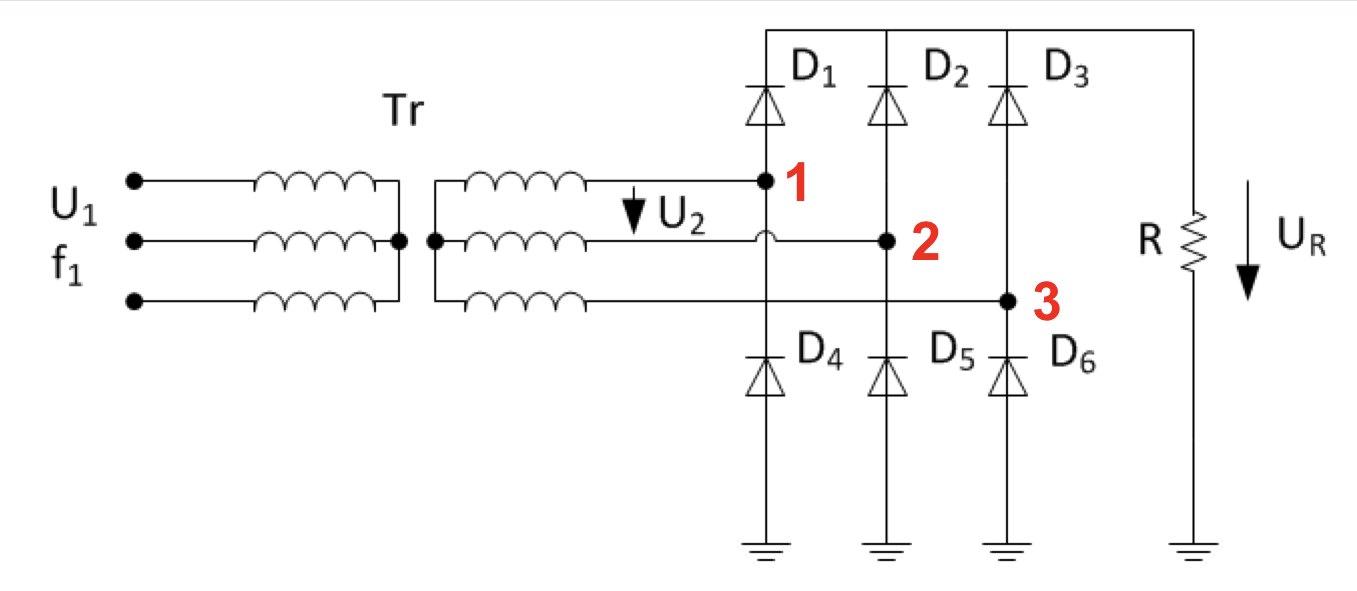
\includegraphics[width=0.65\linewidth]{images/B6U.png}
\end{center}
Zeitverlauf B6U-Gleichrichter:
\begin{center}
    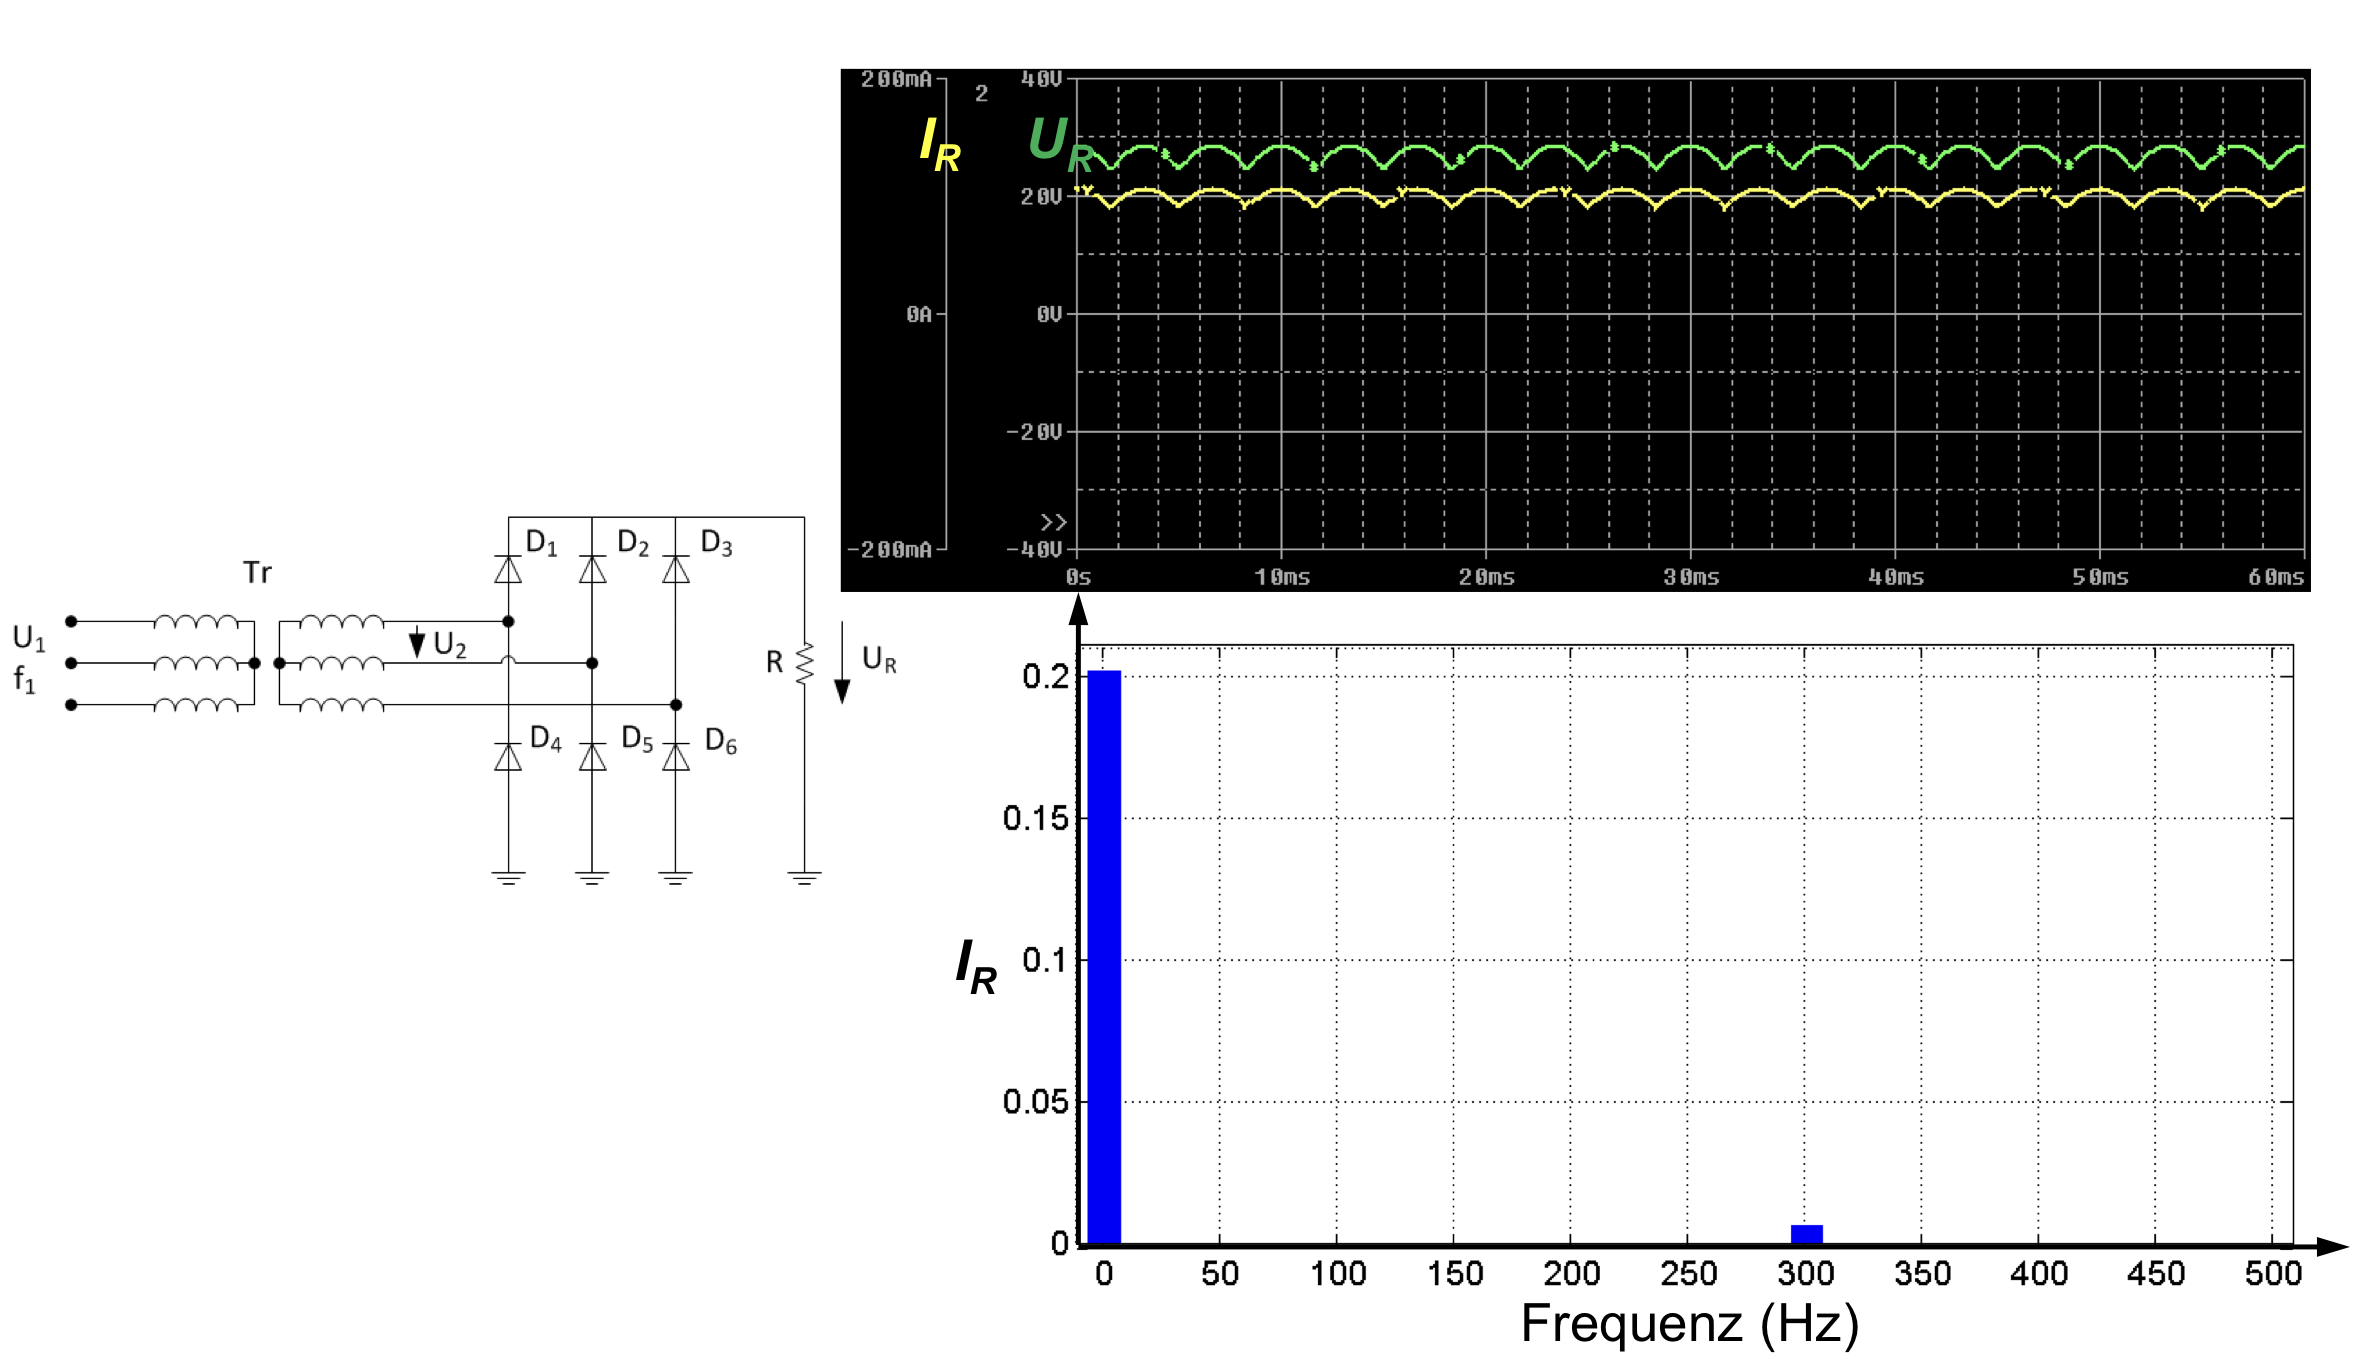
\includegraphics[width=0.85\linewidth]{images/B6U_verlauf.png}
\end{center}
Der B6U-Gleichrichter ist eine dreiphasige Brückenschaltung mit sechs Dioden.
Die Pulszahl beträgt $p=6$.

Mittelwert der Gleichspannung:
\[
\cbl{\overline{u_d} = \frac{3\sqrt{2}}{\pi} U_{LL}}
\]

Eigenschaften:
\begin{itemize}
    \item Sehr geringe Restwelligkeit
    \item Hohe Gleichspannungsqualität
    \item Standard in Industrieanwendungen
\end{itemize}

% -------------------------------------------------

\subsection{B6C: Gesteuerter Dreiphasen-Brückengleichrichter}

% --- bestehende Grafik: B6C Schaltung ---
\begin{center}
    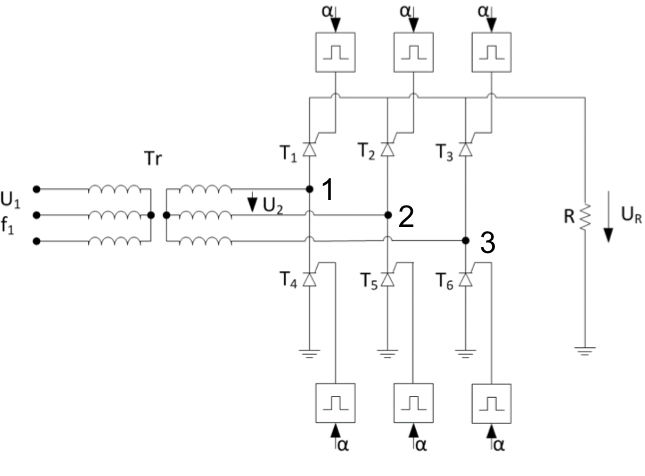
\includegraphics[width=0.65\linewidth]{images/B6C.png}
\end{center}
Zeitverlauf B6C-Gleichrichter:
\begin{center}
    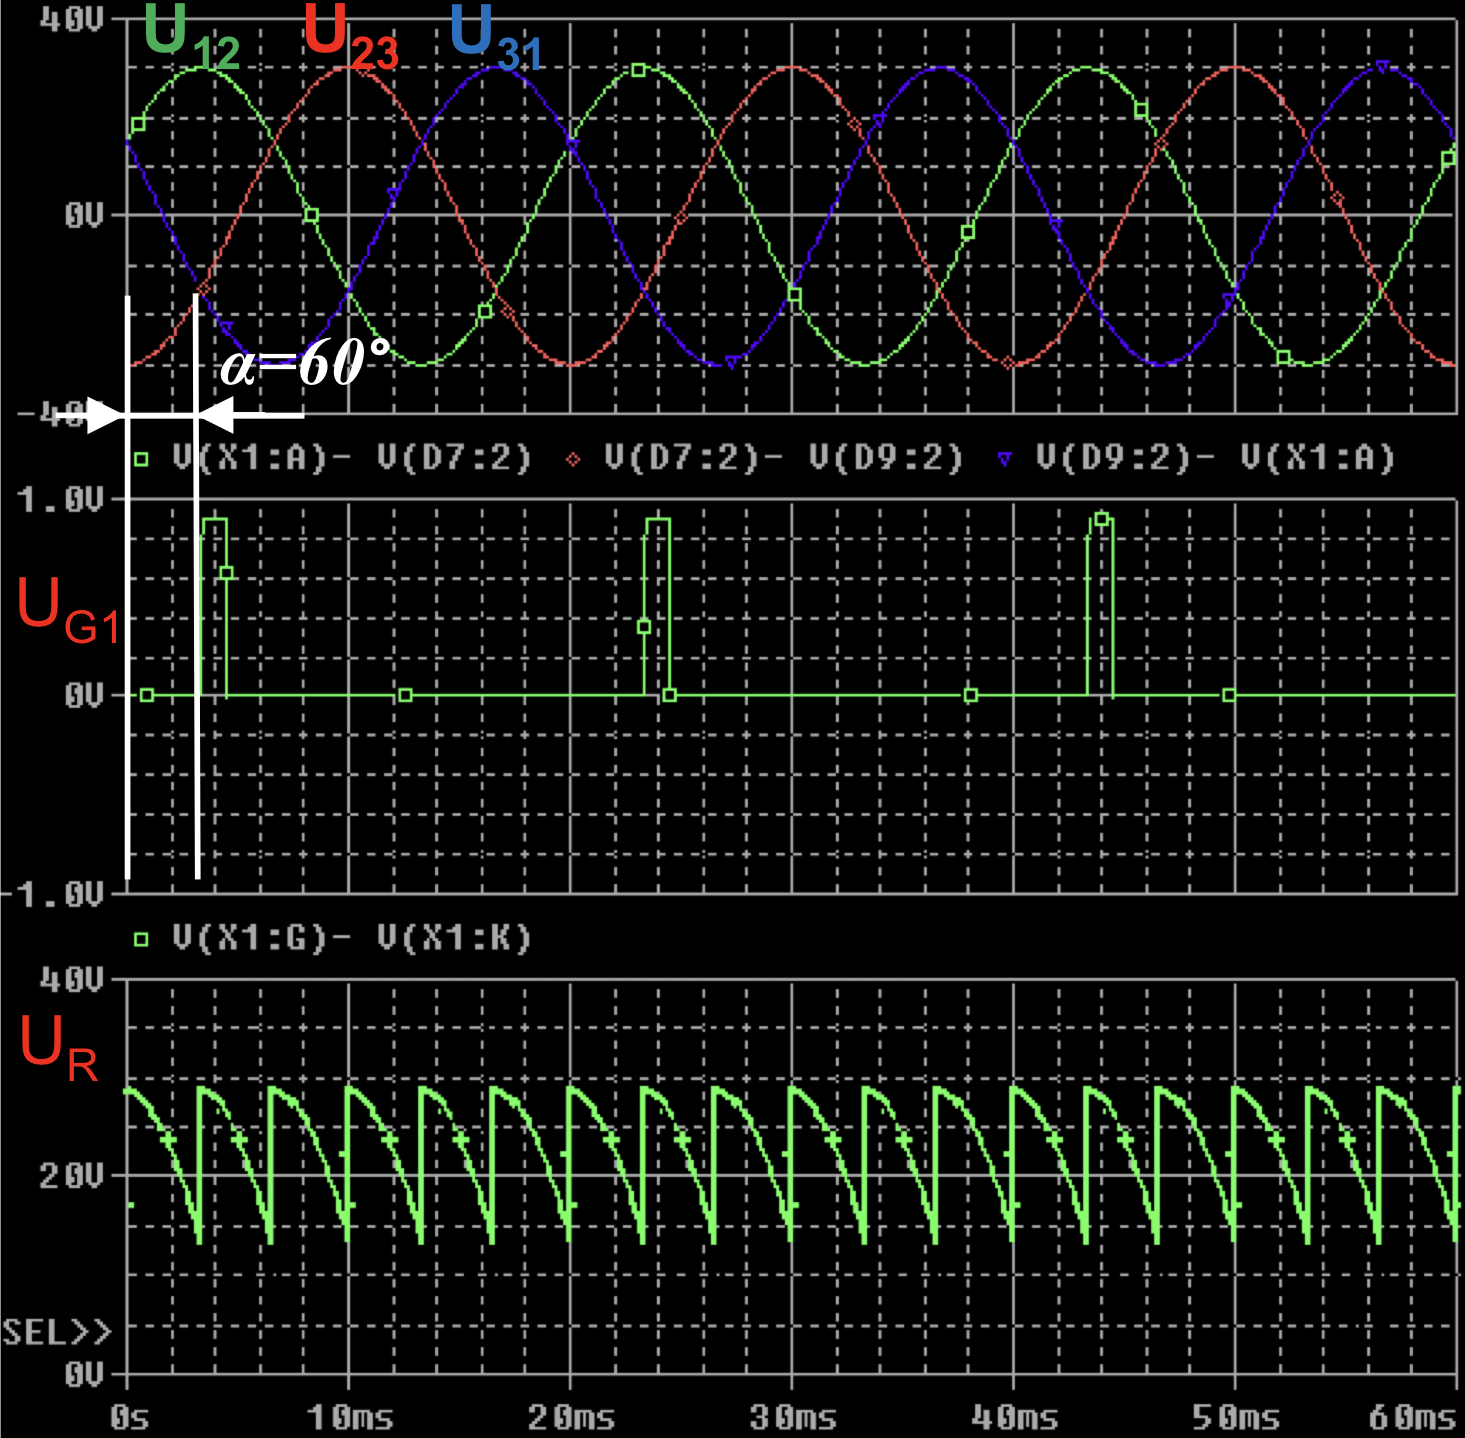
\includegraphics[width=0.85\linewidth]{images/B6C_Verlauf.png}
\end{center}
Beim B6C-Gleichrichter werden die Dioden durch Thyristoren ersetzt.
Die Stellgrösse ist der Zündwinkel $\alpha$.

Mittelwert:
\[
\cbl{\overline{u_d} = \frac{3\sqrt{2}}{\pi} U_{LL} \cos\alpha}
\]

Eigenschaften:
\begin{itemize}
    \item Stellbereich: $0 \le \alpha \le \pi$
    \item Rückspeisebetrieb bei $\alpha > 90^\circ$
    \item Vierquadrantenbetrieb möglich
\end{itemize}

% -------------------------------------------------

\subsection{Kommutierungsüberlappung}

% --- bestehende oder neue Grafik: Überlappung ---
\begin{figure}[h]
\centering
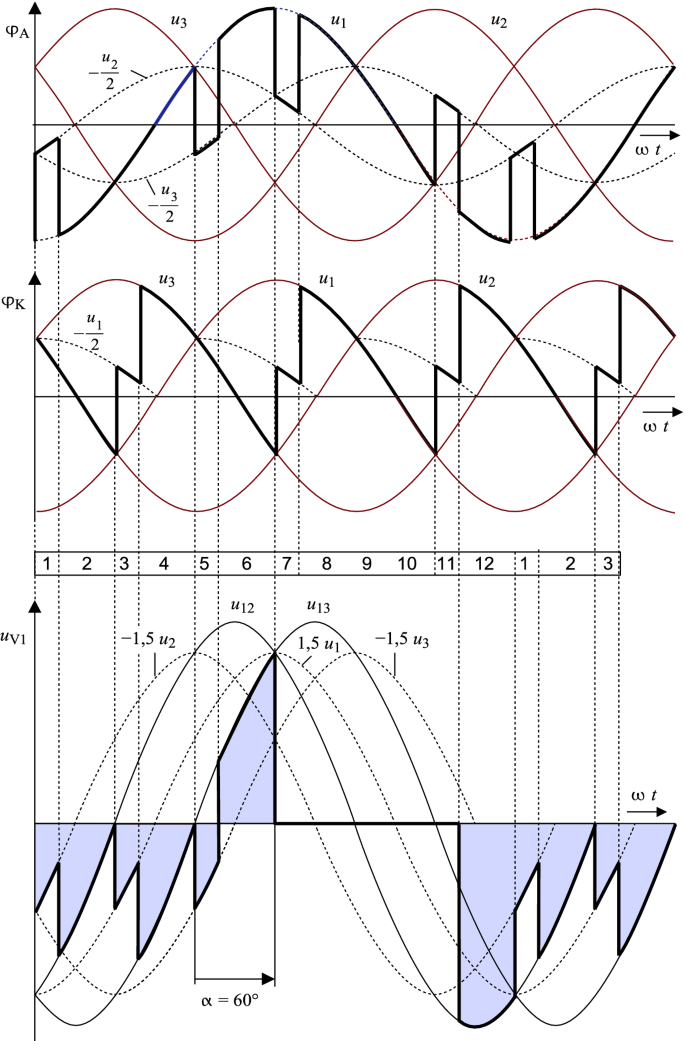
\includegraphics[width=0.65\linewidth]{images/kommutierung.png}
\caption{Kommutierungsüberlappung $\mu$ beim B6-Gleichrichter}
\end{figure}

In realen Netzen ist die Netzinduktivität $L_\sigma$ nicht null.
Dadurch kann der Strom nicht sprunghaft umschalten.
Während der Überlappung leiten \textbf{drei} Ventile gleichzeitig.

Grundgleichung:
\[
\cbl{u_\sigma(t) = L_\sigma \frac{di(t)}{dt}}
\]

Spannungsabfall:
\[
\cbl{\Delta u_d \propto \omega L_\sigma i_d}
\]

Aussage:
\begin{itemize}
    \item $L_\sigma \uparrow \Rightarrow \overline{u_d} \downarrow$
    \item $i_d \uparrow \Rightarrow \overline{u_d} \downarrow$
\end{itemize}

\paragraph{Überlappungsverlust bei Netzinduktivität}
Bei endlicher Netzinduktivität $L_\sigma$ ergibt sich ein zusätzlicher Spannungsabfall:
\[
\Delta u_d = \frac{3}{\pi} \, \omega L_\sigma i_d
\]
Damit:
\[
u_d = \frac{3\sqrt{2}}{\pi} U_{LL} \cos\alpha - \Delta u_d
\]


% -------------------------------------------------

\subsection{Netzströme und Harmonische}

% --- bestehende Grafik: Netzstrom ---
\begin{figure}[h]
\centering
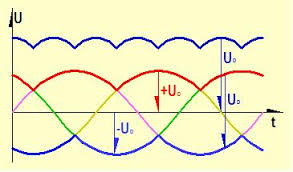
\includegraphics[width=0.7\linewidth]{images/B6strom.png}
\caption{Leiterstrom beim B6-Gleichrichter}
\end{figure}

Bei grosser Glättinduktivität ist der Gleichstrom $i_d$ näherungsweise konstant.
Die Leiterströme sind rechteckförmig (120$^\circ$-Leitung).

Harmonische Ordnung:
\[
\cbl{n = 6k \pm 1 \qquad (k \in \mathbb{N})}
\]

Dominant:
\[
\cbl{5,\;7,\;11,\;13,\;\dots}
\]

Nicht vorhanden:
\[
\cbl{3,\;9,\;15,\;\dots}
\]

% -------------------------------------------------

\subsection{Vergleich B2 -- B6}

\begin{center}
\begin{tabular}{l|c|c}
 & B2 & B6 \\ \hline
Pulszahl & 2 & \cbl{6} \\
Restwelligkeit & hoch & \cbl{gering} \\
Gleichspannungsqualität & gering & \cbl{hoch} \\
Netzstrom & stärker verzerrt & \cbl{weniger verzerrt} \\
\end{tabular}
\end{center}

\subsection{Merksätze}

\begin{itemize}
    \item B6 ist der wichtigste industrielle Gleichrichter.
    \item Mittelwert proportional zu $\cos\alpha$ beim B6C.
    \item Netzstromharmonische: $6k \pm 1$.
\end{itemize}
